\documentclass[11pt,a4paper]{article}

\usepackage[margin=1in]{geometry}
\usepackage{amsmath,amssymb,amsfonts}
\usepackage{graphicx}
\usepackage{booktabs}
\usepackage{hyperref}
\usepackage{caption}
\usepackage{subcaption}
\usepackage{microtype}
\usepackage{cite}
\usepackage{xcolor}

\hypersetup{
    colorlinks=true,
    linkcolor=blue!70!black,
    citecolor=green!50!black,
    urlcolor=blue!80!black
}

\title{\textbf{Physical Invariants and Failure-Mode Error Predictability in Diffusion Emulators for Pseudo-Relativistic $N$-Body Dynamics}}

\author{
    \textbf{Kartik Sirohi} \\
    \texttt{sirohikartik@gmail.com}
}

\date{\today}

\begin{document}

\maketitle

\begin{abstract}
Diffusion models offer a computationally efficient approach to emulating dynamical systems, but their autoregressive rollouts can violate physical structure and accumulate prediction errors. We study internal representations and failure modes in conditional diffusion emulators trained on pseudo-relativistic Barnes-Hut $N$-body trajectories. We evaluate four denoiser widths, $d \in \{32,64,128,256\}$, using linear probes for physical quantities and probes for future transition error. Increasing width substantially improves linear accessibility of angular momentum, with $R^2$ increasing from 0.255 to 0.934, and generally improves energy accessibility. However, this improvement does not translate into more stable autoregressive rollouts: 30-step RMSE increases from 6.966 at $d=32$ to 18.465 at $d=256$, despite lower validation loss. For a $d=128$ model, transition error is linearly predictable from intermediate activations, reaching Pearson $r=0.6852$ at the pre-head layer. Comparing low- and high-error transitions shows a 35.6\% reduction in position decodability and an 11.9\% reduction in angular-momentum decodability during failures. Ensemble predictive spread correlates with transition error but does not reliably detect abrupt strong-field failures. These results show that physical information accessibility, one-step prediction quality, and long-horizon stability can diverge in diffusion-based physics emulators.
\end{abstract}

\section{Introduction}
Modeling self-gravitating astrophysical phenomena around supermassive black holes (SMBHs)—such as plasma accretion disks and tidal disruption events—is a cornerstone of computational astrophysics. Direct $N$-body integration scales quadratically ($O(N^2)$), creating a computational bottleneck. To alleviate this, hierarchical spatial approximations such as the 3D Barnes-Hut octree \cite{sanchez-gonzalez2020learning} approximate distant particle clusters using multipole center-of-mass moments, reducing the cost to $O(N \log N)$. Furthermore, incorporating strong-field gravitational features—such as event horizon capture and the Innermost Stable Circular Orbit (ISCO)—without the prohibitive computational cost of numerical relativity is typically achieved via pseudo-Newtonian prescriptions like the Paczy\'nski--Wiita potential.

Despite these algorithmic advances, high-resolution multi-step numerical integration remains computationally demanding and inherently sequential. Recently, deep learning surrogates and neural dynamical emulators have gained widespread interest across physical sciences. Early efforts predominantly focused on graph neural networks (GNNs) \cite{sanchez-gonzalez2020learning} to learn mesh-free particle interactions. More recently, conditional denoising diffusion probabilistic models have emerged as state-of-the-art generative emulators across weather forecasting and turbulent fluid dynamics \cite{finn2024representation, li2024generative, bastek2024physics}. Diffusion models offer the distinct advantage of stochastic ancestral sampling, enabling the generation of forecast ensembles that capture ensemble predictive spread in chaotic phase spaces.

Nonetheless, critical questions remain regarding the deployment of diffusion emulators for dynamical systems:
\begin{enumerate}
    \item \textbf{Representation Capacity vs. Rollout Reliability:} Does increasing denoiser width and improving physical invariant decodability yield more stable autoregressive rollouts, or do one-step objective optimization and multi-step dynamical stability diverge?
    \item \textbf{Failure Mode Representation Breakdown:} When the emulator makes incorrect predictions—such as near the strong-field ISCO regime—how do internal geometric representations degrade?
    \item \textbf{Error Predictability and Latent Diagnostics:} Can intermediate layer activations linearly predict future transition error, and does this predictive capacity provide information beyond what is already determined by the input physical state?
\end{enumerate}

In this paper, we address these questions by combining conditional diffusion emulators with mechanistic representation probing techniques. Inspired by diagnostic probing in computer vision and natural language processing \cite{kim2018interpretability, zhang2024best, geiger2023causal, rozet2025lost}, we train linear probes on intermediate activations to evaluate the accessibility of physical invariants, analyze error predictability, and study representation degradation during failure.

\section{Related Work}
\label{sec:related_work}

\paragraph{Graph Networks for Physical Simulation.}
Sanchez-Gonzalez et al. \cite{sanchez-gonzalez2020learning} demonstrated that graph neural networks (GNNs) with message-passing architectures can approximate complex fluid, rigid body, and deformable material interactions. In their framework, an encoder maps particle states into a latent interaction graph, a processor executes multi-step relational message-passing, and a decoder outputs kinematic updates (such as accelerations). While GNNs enforce spatial permutation equivariance, their rollout stability depends heavily on artificial noise injection during training, and direct evaluation of strong-field relativistic potentials remains challenging.

\paragraph{Diffusion Models for Dynamical Systems.}
Denoising diffusion models have recently demonstrated remarkable performance in emulating continuous physical processes. Finn et al. \cite{finn2024representation} established that unconditional diffusion models trained on dynamical systems develop rich internal representations of underlying attractors. By probing frozen features with linear regression heads, they showed that diffusion latents capture system state coordinates and can produce predictive ensembles. Similarly, Li et al. \cite{li2024generative} utilized diffusion models conditioned on classical physics simulation seeds to generate high-fidelity weather forecast ensembles, matching traditional numerical weather prediction ensembles at reduced computational cost. Furthermore, Bastek et al. \cite{bastek2024physics} introduced physics-informed diffusion formulations, incorporating differential equation residuals into score-based sampling objectives.

\paragraph{Representational Vulnerabilities in Dynamical Emulators.}
Despite their expressive power, generative emulators exhibit distinct failure modes. Rozet et al. \cite{rozet2025lost} conducted an empirical study on latent diffusion models for physics emulation, identifying that compressed autoencoding representations frequently struggle with out-of-distribution phase drift, information bottleneck loss, and non-physical energy divergence. These limitations underscore the necessity of inspecting what features neural emulators actually encode and how representations behave when predictions fail.

\paragraph{Mechanistic Interpretability and Representation Probing.}
Understanding internal neural mechanisms has advanced through targeted probing and causal interventions. Kim et al. \cite{kim2018interpretability} introduced Testing with Concept Activation Vectors (TCAV), providing a quantitative framework to determine whether human-interpretable concepts are linearly represented in intermediate network layers. In language models, Zhang and Nanda \cite{zhang2024best} developed activation patching paradigms to isolate the precise layers responsible for specific computational behaviors by intervening on clean versus corrupted execution paths. Formally uniting these approaches, Geiger et al. \cite{geiger2023causal} formalized causal abstraction, establishing a mathematical framework relating high-level causal causal variables to low-level neural representations. In this work, we build on these foundations to develop a physical probing and self-diagnosis suite for diffusion emulators.

\section{Methodology}

\subsection{Pseudo-Relativistic \texorpdfstring{$N$}{N}-Body Ground Truth Simulator}
The ground truth dynamics are generated by a C++17 simulation core featuring a central supermassive black hole of mass $M_{\mathrm{BH}}$ surrounded by $N$ orbiting bodies. Spatial acceleration is governed by two interacting components:

\paragraph{Paczy\'nski--Wiita Central Potential.}
To model Schwarzschild relativistic dynamics without the extreme computational overhead of full numerical relativity, the central gravitational field uses the Paczy\'nski--Wiita pseudo-Newtonian prescription:
\begin{equation}
    \Phi_{\mathrm{PW}}(r) = -\frac{G M_{\mathrm{BH}}}{r - r_s}, \qquad \vec{a}_{\mathrm{PW}}(r) = -\frac{G M_{\mathrm{BH}}}{(r - r_s)^2} \frac{\vec{r}}{r}, \quad (r > r_s),
\end{equation}
where $r_s = \frac{2 G M_{\mathrm{BH}}}{c^2}$ is the Schwarzschild event horizon radius. This formulation reproduces key relativistic orbital features, notably the photon sphere at $r_{\mathrm{ph}} = 1.5 r_s$ and the Innermost Stable Circular Orbit at $r_{\mathrm{ISCO}} = 3.0 r_s$, inside which circular orbits become dynamically unstable and plunge inward. 

\paragraph{Integrator \& Non-Hamiltonian Horizon Capture.}
Pairwise interactions among the $N$ orbiting bodies are calculated using a 3D Barnes-Hut octree with a multipole opening angle criterion $\theta = 0.6$ and Plummer softening parameter $\epsilon = 0.08$:
\begin{equation}
    \vec{a}_{ij} = \frac{G m_j (\vec{r}_j - \vec{r}_i)}{\left(\|\vec{r}_j - \vec{r}_i\|^2 + \epsilon^2\right)^{3/2}}.
\end{equation}
Velocity-Verlet time integration is used for the smooth orbital dynamics, preserving phase-space volume along conservative trajectories:
\begin{align}
    \vec{x}(t + \Delta t) &= \vec{x}(t) + \vec{v}(t)\Delta t + \frac{1}{2}\vec{a}(t)\Delta t^2, \\
    \vec{v}(t + \Delta t) &= \vec{v}(t) + \frac{1}{2}\Big(\vec{a}(t) + \vec{a}(t + \Delta t)\Big)\Delta t.
\end{align}
Particles entering $r \le r_s$ undergo inelastic horizon capture. Crucially, while Velocity-Verlet preserves phase-space volume for continuous Hamiltonian dynamics, horizon capture introduces a non-Hamiltonian termination event that abruptly alters particle count and total momentum.

\subsection{Conditional Diffusion Physics Emulator}
Let $x_t \in \mathbb{R}^D$ denote the full physical state vector at timestep $t$, containing coordinates and velocities for all bodies and the black hole:
\begin{equation}
    x_t = [\mathbf{p}_1, \mathbf{v}_1, \dots, \mathbf{p}_N, \mathbf{v}_N, \mathbf{p}_{\mathrm{BH}}, \mathbf{v}_{\mathrm{BH}}], \quad D = 6N + 6.
\end{equation}
Rather than predicting future state $x_{t+1}$ directly, our emulator targets the normalized displacement $\Delta x_t = x_{t+1} - x_t$. The conditional denoiser $\epsilon_\theta(y_k, k, x_t)$ is parameterized by a lightweight residual architecture featuring sinusoidal timestep embeddings, input LayerNorm, and a sequence of residual blocks. 

The forward diffusion process corrupts target state displacement $y_0 = \Delta x_t$ over $K$ discrete timesteps:
\begin{equation}
    q(y_k \mid y_0) = \mathcal{N}\left(y_k; \sqrt{\bar{\alpha}_k} y_0, (1 - \bar{\alpha}_k) \mathbf{I}\right),
\end{equation}
where $\bar{\alpha}_k = \prod_{s=1}^k (1 - \beta_s)$. The network is trained using the standard mean squared error objective:
\begin{equation}
    \mathcal{L}(\theta) = \mathbb{E}_{k, y_0, \epsilon}\left[\|\epsilon - \epsilon_\theta(y_k, k, x_t)\|^2\right].
\end{equation}
During inference, given condition state $x_t$, ancestral sampling iteratively inverts the noise from $y_K \sim \mathcal{N}(0, \mathbf{I})$ down to $y_0 = \Delta \hat{x}_t$, yielding $\hat{x}_{t+1} = x_t + \Delta \hat{x}_t$. Generating $S$ stochastic paths provides an ensemble $\{\hat{x}_{t+1}^{(s)}\}_{s=1}^S$ whose variance measures ensemble predictive spread.

\subsection{Physical Probing and Diagnostic Framework}

\paragraph{Layer Representation Extraction.}
To inspect internal mechanics, we extract intermediate activation representations $h_l(x_t)$ across the denoiser:
\begin{equation}
    h_l \in \{ h_{\mathrm{input}}, h_1, h_2, h_3, h_{\mathrm{pre\_head}} \}.
\end{equation}

\paragraph{Invariant Decodability Probing.}
For each internal layer $h_l$, we train a cross-validated linear Ridge regression probe $f_l(h) = \mathbf{W}_l h + \mathbf{b}_l$ to predict ground truth physical properties $y_{\mathrm{phys}}$:
\begin{equation}
    y_{\mathrm{phys}} \in \left\{ E_{\mathrm{total}}, \|\vec{L}\|, \|\vec{P}\|, \mathbf{p}, \mathbf{v}, U_{\mathrm{potential}}, K_{\mathrm{kinetic}} \right\}.
\end{equation}
Probing performance is evaluated on held-out test transitions using the coefficient of determination ($R^2$), root mean squared error (RMSE), and Pearson correlation ($r$). A high $R^2$ indicates that the physical quantity is linearly accessible within that representation subspace.

\paragraph{Error Predictability and State-Controlled Baselines.}
To test whether internal representations encode impending prediction error, we fit linear probes on $h_l$ to predict the single-step rollout error magnitude $e_{\mathrm{actual}} = \|\Delta \hat{x}_{t+1} - \Delta x_{t+1}^{\mathrm{GT}}\|$. However, because certain physical states (e.g., proximity to the ISCO) are intrinsically harder to predict, a probe correlating with error could merely reflect input state difficulty rather than model-specific error encoding. To address this, we implement two explicit baselines:
\begin{enumerate}
    \item \textbf{Physical Feature Baseline:} Linear probe using geometric features: minimum distance to SMBH $r_{\min}/r_s$, mean and maximum body velocities, total angular momentum $\|\vec{L}\|$, and distance to the ISCO $|r_{\min} - r_{\mathrm{ISCO}}|$.
    \item \textbf{Raw Input State Baseline:} Linear probe directly mapping full raw coordinates $x_t \longrightarrow e_{\mathrm{actual}}$.
\end{enumerate}
Furthermore, we evaluate residualized error prediction:
\begin{equation}
    e_{\mathrm{res}} = e_{\mathrm{actual}} - \hat{e}_{\mathrm{baseline}}(x_t),
\end{equation}
testing whether $h_{\mathrm{pre\_head}}$ predicts residual error $e_{\mathrm{res}}$ after linearly regressing out the physical input state $x_t$.

\paragraph{Regime Dissection.}
To evaluate representational degradation during failure, held-out test transitions ($n=331$) are partitioned into:
\begin{itemize}
    \item \textbf{Success Regime ($n=83$):} Transitions in the lowest quartile of prediction error ($e \le 1.0104$).
    \item \textbf{Failure Regime ($n=83$):} Transitions in the highest quartile of prediction error ($e \ge 1.6038$).
\end{itemize}
Thresholds are computed strictly on the held-out test set from trajectories unseen during training. Invariant probing is evaluated across both subsets, reporting $\Delta R^2 = R^2_{\mathrm{succ}} - R^2_{\mathrm{fail}}$.

\begin{figure*}[t]
    \centering
    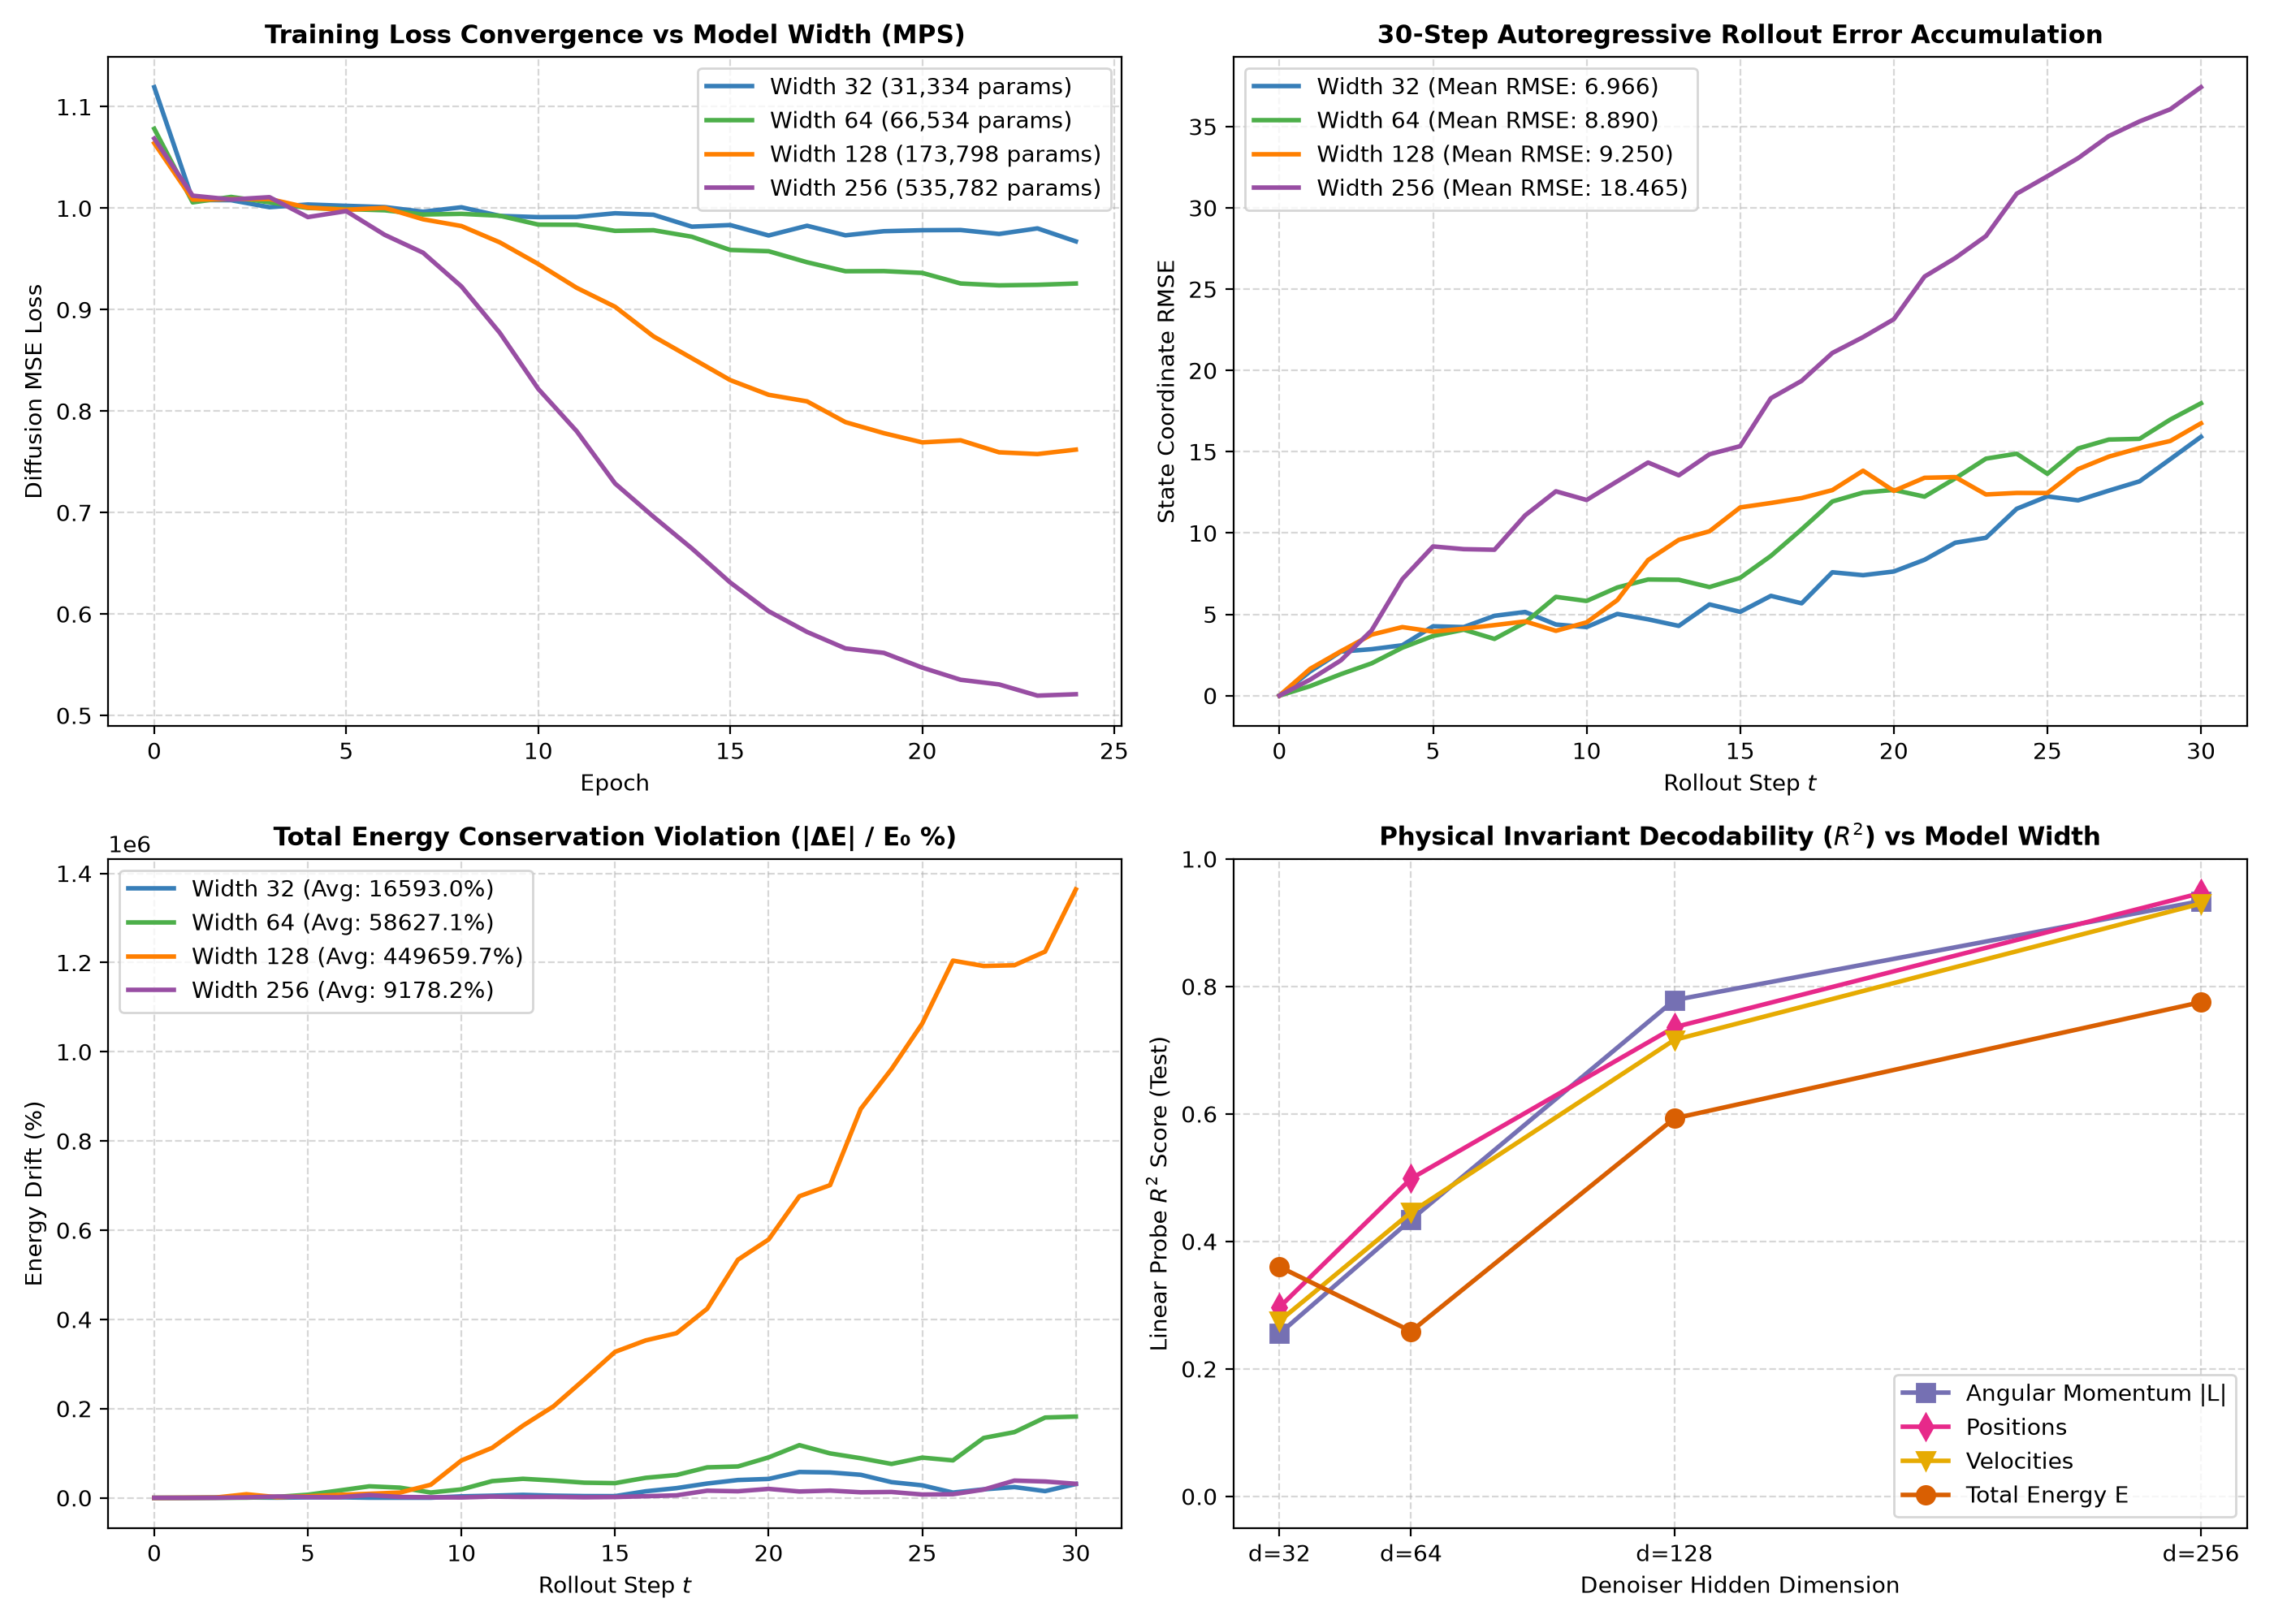
\includegraphics[width=\textwidth]{experiments_output/model_width_comparison.png}
    \caption{\textbf{Diffusion Model Width Scaling Study.} (Top-Left) Diffusion MSE training loss convergence across widths $d \in \{32, 64, 128, 256\}$. (Top-Right) 30-step autoregressive rollout RMSE accumulation. (Bottom-Left) Secular total energy conservation violation drift ($|\Delta E|/E_0$). (Bottom-Right) Linear probe $R^2$ scores for physical invariants as a function of denoiser width.}
    \label{fig:width_scaling}
\end{figure*}

\section{Experimental Results}

\subsection{Experimental Setup \& Compute Efficiency}
All experiments were executed on an Apple Silicon M1 (8 GB unified memory) utilizing the Metal Performance Shaders (MPS) PyTorch backend. The dataset comprises 30 pseudo-relativistic Barnes-Hut trajectories of 60 steps each ($N=16$ bodies, state dimension $D=102$, $\Delta t = 0.01$). Two complete trajectories are reserved strictly for continuous autoregressive rollout evaluation. Training each model configuration required between $4.7$ and $5.4$ seconds on Apple Silicon MPS, with inference latency ranging from $13.5$ to $18.5$ ms per diffusion rollout step. Because consecutive steps within an astrophysical trajectory share dynamical history, these empirical results illustrate representative scaling behaviors under fixed resources; future studies should evaluate multi-seed confidence intervals across expanded trajectory distributions.

\subsection{Experiment 1: Diffusion Model Width Scaling Study}
We investigated four denoiser widths: $d=32$ ($31\text{k}$ parameters), $d=64$ ($66\text{k}$ parameters), $d=128$ ($174\text{k}$ parameters), and $d=256$ ($536\text{k}$ parameters). Quantitative results are summarized in Table~\ref{tab:width_scaling} and visualized in Figure~\ref{fig:width_scaling}.

\begin{table}[t]
\centering
\small
\caption{\textbf{Quantitative Comparison across Diffusion Denoiser Hidden Dimensions ($d$).} Metrics include parameter counts, single-step convergence losses, 30-step autoregressive rollout RMSE, linear probe decodability ($R^2$ on held-out test data from intermediate layer $h_2$), single-step rollout latency, and training duration on Apple Silicon MPS.}
\label{tab:width_scaling}
\resizebox{\columnwidth}{!}{
\begin{tabular}{lcccccccc}
\toprule
\textbf{Width ($d$)} & \textbf{Params} & \textbf{Train Loss} & \textbf{Val Loss} & \textbf{Rollout RMSE} & \textbf{Energy $R^2$} & \textbf{Ang. Mom. $R^2$} & \textbf{Latency} & \textbf{Train Time} \\
\midrule
$d = 32$  & 31,334  & 0.9673 & 0.9875 & \textbf{6.966} & 0.3602 & 0.2553 & 14.5 ms & 4.89 s \\
$d = 64$  & 66,534  & 0.9258 & 0.9169 & 8.890          & 0.2590 & 0.4342 & 17.0 ms & 4.73 s \\
$d = 128$ & 173,798 & 0.7620 & 0.7786 & 9.250          & 0.5930 & 0.7785 & \textbf{13.5 ms} & 4.71 s \\
$d = 256$ & 535,782 & \textbf{0.5209} & \textbf{0.5311} & 18.465 & \textbf{0.7754} & \textbf{0.9340} & 18.5 ms & 5.38 s \\
\bottomrule
\end{tabular}
}
\end{table}

\paragraph{Physical Invariant Decodability Across Widths.}
As illustrated in Figure~\ref{fig:width_scaling} (bottom-right), increasing network width generally improves the linear decodability of physical invariants. For angular momentum ($\|\vec{L}\|$), we observe a strict monotonic increase in probe $R^2$ across all widths: $0.2553$ ($d=32$), $0.4342$ ($d=64$), $0.7785$ ($d=128$), and $0.9340$ ($d=256$)—a $+266\%$ cumulative gain. Total energy accessibility also improves substantially overall from $0.3602$ at $d=32$ to $0.7754$ at $d=256$ ($+115\%$ gain), despite a slight non-monotonic dip at $d=64$ ($R^2 = 0.2590$). Coordinate decodability scales monotonically from $R^2 = 0.2968$ to $0.9466$. This demonstrates that expanded representation capacity structures the latent manifold so that physical quantities become linearly accessible.

\paragraph{Tension Between Single-Step Loss and Autoregressive Rollout Stability.}
The most significant scientific result in Table~\ref{tab:width_scaling} is the stark divergence between single-step training accuracy and continuous autoregressive rollout stability. At width $d=256$, the model fits the single-step training objective much better, cutting training MSE loss to $0.5209$ and validation MSE loss to $0.5311$ (a $46.2\%$ reduction compared to $d=32$). However, over a 30-step continuous autoregressive rollout, its RMSE surges to $18.465$. In sharp contrast, the narrowest model ($d=32$) exhibits substantially higher single-step loss ($0.9673$ train, $0.9875$ validation), yet produces a much more stable rollout with an RMSE of only $6.966$ (a $62.3\%$ reduction in trajectory error relative to $d=256$). In the absence of symplectic or Hamiltonian structural constraints, highly parameterized unconstrained denoisers fit high-frequency residuals that compound during recursive autoregression, inducing rapid phase drift.

\begin{figure*}[t]
    \centering
    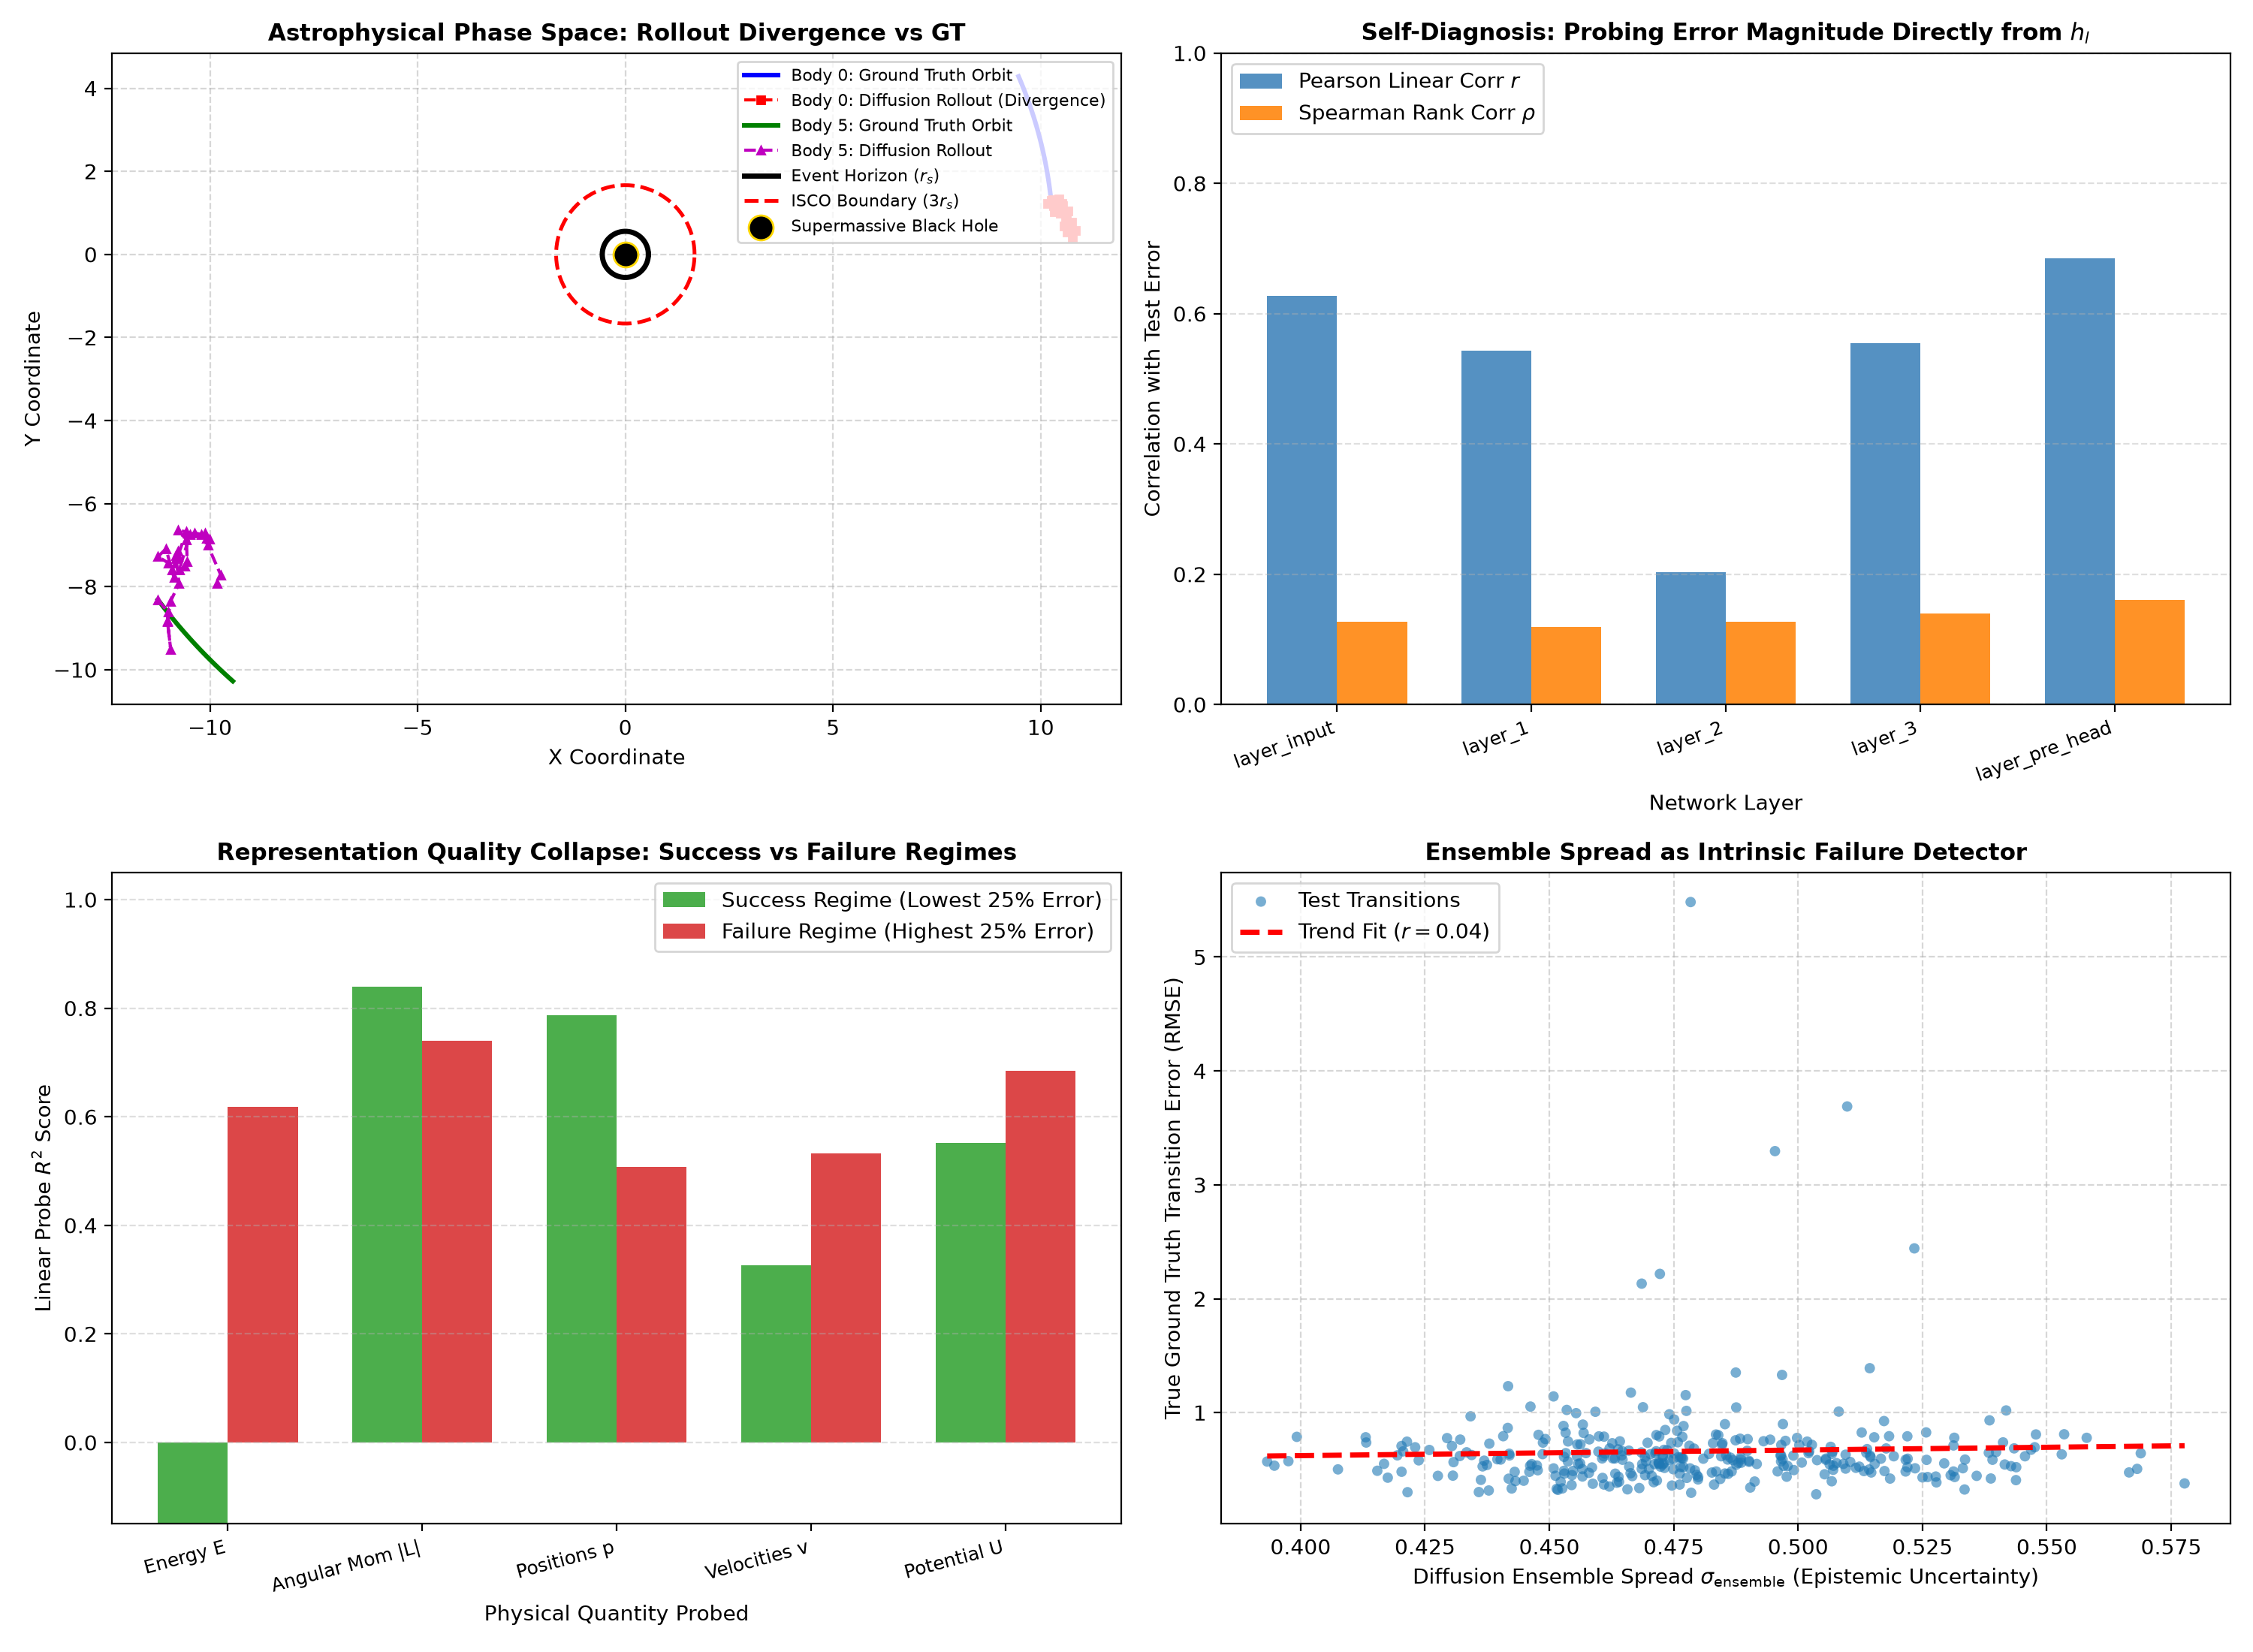
\includegraphics[width=\textwidth]{experiments_output/failure_mode_probing.png}
    \caption{\textbf{Probing Failure Modes and Representation Breakdown.} (Top-Left) Phase-space trajectory showing ground truth orbit and diffusion rollout divergence near the Schwarzschild horizon ($r_s$) and ISCO ($3 r_s$). (Top-Right) Error Predictability Probing: Pearson linear correlation ($r$) and Spearman rank correlation ($\rho$) predicting transition error magnitude from intermediate layers $h_l$ and baselines. (Bottom-Left) Representation quality degradation in Success (lowest 25\% error) vs. Failure (highest 25\% error) regimes. (Bottom-Right) Ensemble predictive spread ($\sigma_{\mathrm{ensemble}}$) versus true transition error.}
    \label{fig:failure_probing}
\end{figure*}

\subsection{Experiment 2: Probing Failure Modes and Error Predictability}
Using the flagship model ($d=128$), we probed internal representation behaviors during prediction failures. Results are visualized in Figure~\ref{fig:failure_probing}.

\paragraph{Astrophysical Anatomy of Failure.}
As depicted in Figure~\ref{fig:failure_probing} (top-left), severe failure modes occur primarily in two regimes: (1) orbital phase divergence during extended multi-step rollouts, and (2) close encounters within the strong-field region $r \le 3.0 r_s$. Near the ISCO boundary, steep gravitational gradients amplify coordinate under-predictions, triggering artificial inward plunge toward the black hole.

\paragraph{Error Predictability and State-Controlled Baselines.}
Can intermediate layer representations predict upcoming transition errors before coordinate projection? Table~\ref{tab:error_predictability} and Figure~\ref{fig:failure_probing} (top-right) report probe correlations across layers and comparison baselines. Linear probes trained on intermediate activations achieve substantial correlation with future transition error, reaching $r = 0.6268$ at $h_{\mathrm{input}}$ and peaking at **$r = 0.6852$** at the pre-head layer $h_{\mathrm{pre\_head}}$. 

Crucially, because strong-field orbital configurations near the ISCO are intrinsically more difficult to integrate, we evaluate whether this correlation simply reflects input state difficulty. Probing simple physical features ($r_{\min}/r_s$, velocity, $\|\vec{L}\|$, and ISCO distance) directly yields $r = 0.7467$ ($R^2 = 0.5486$), while the raw state baseline $x_t$ yields $r = 0.4639$ ($R^2 = 0.2139$). This confirms that physical state difficulty accounts for a significant portion of error predictability.

To test whether hidden representations contain model-specific predictive information beyond the physical input state, we trained a linear probe on $h_{\mathrm{pre\_head}}$ to predict the residualized error $e_{\mathrm{res}} = e_{\mathrm{actual}} - \hat{e}_{\mathrm{baseline}}(x_t)$. The probe achieves a Pearson correlation of $r = 0.4318$ ($\rho = 0.1905$) on the residualized error. This demonstrates that internal activations carry predictive error information beyond the geometry of the input state.

Across layers, error predictability exhibits a non-monotonic pattern: correlation dips at $h_2$ ($r = 0.2031$) before recovering at $h_3$ ($r = 0.5542$) and peaking at $h_{\mathrm{pre\_head}}$ ($r = 0.6852$), reflecting the transition from relational coordinate processing to final displacement estimation.

\begin{table}[h]
\centering
\small
\caption{\textbf{Error Predictability Probing across Layers and Baselines.} Linear probe Pearson correlation ($r$), Spearman rank correlation ($\rho$), and held-out test $R^2$ predicting single-step ground truth transition error magnitude directly from internal activations $h_l$ and state baselines.}
\label{tab:error_predictability}
\resizebox{\columnwidth}{!}{
\begin{tabular}{lcccl}
\toprule
\textbf{Representation / Feature} & \textbf{Pearson ($r$)} & \textbf{Spearman ($\rho$)} & \textbf{Test $R^2$} & \textbf{Diagnostic Role} \\
\midrule
Physical Features ($r_{\min}, v, \|\vec{L}\|, d_{\mathrm{ISCO}}$) & \textbf{0.7467} & \textbf{0.1972} & \textbf{0.5486} & Physical difficulty baseline \\
Raw Input State ($x_t \in \mathbb{R}^{102}$)            & 0.4639 & 0.1359 & 0.2139 & Kinematic state baseline \\
\midrule
Layer $h_{\mathrm{input}}$                               & 0.6268 & 0.1264 & -4.099 & Initial geometric projection \\
Layer $h_1$                                              & 0.5437 & 0.1190 & -4.819 & Relational spatial tracking \\
Layer $h_2$                                              & 0.2031 & 0.1255 & -3.577 & Non-linear feature transformation \\
Layer $h_3$                                              & 0.5542 & 0.1388 & -3.572 & Non-monotonic error recovery \\
Layer $h_{\mathrm{pre\_head}}$                           & \textbf{0.6852} & 0.1601 & -4.291 & Peak activation correlation \\
\midrule
Residualized ($h_{\mathrm{pre\_head}} \to e_{\mathrm{res}}$) & 0.4318 & 0.1905 & --- & Signal beyond input state \\
\bottomrule
\end{tabular}
}
\end{table}

\paragraph{Representation Breakdown during Failure.}
Partitioning the 331 held-out test transitions into success ($n=83$, $e \le 1.0104$) and failure ($n=83$, $e \ge 1.6038$) regimes reveals marked representational asymmetry (Figure~\ref{fig:failure_probing}, bottom-left). In successful transitions, position decodability is robust ($R^2 = 0.7869$), and angular momentum is preserved ($R^2 = 0.8397$). During failure, position decodability drops by **$35.6\%$** ($R^2$ collapses to $0.5069$), and angular momentum drops to $0.7400$ ($11.9\%$ reduction). 

Importantly, this representational degradation is accompanied by physical state shift: in the failure group, mean $r_{\min}$ drops to $2.582$ with $8.4\%$ of states reaching within the ISCO ($r \le 3.0 r_s$), whereas the success group has mean $r_{\min} = 2.848$ with $0\%$ near the ISCO. This demonstrates that model failure is associated with both coordinate representation degradation and strong-field gravitational shear.

\begin{figure*}[t]
    \centering
    \begin{subfigure}[b]{0.49\textwidth}
        \centering
        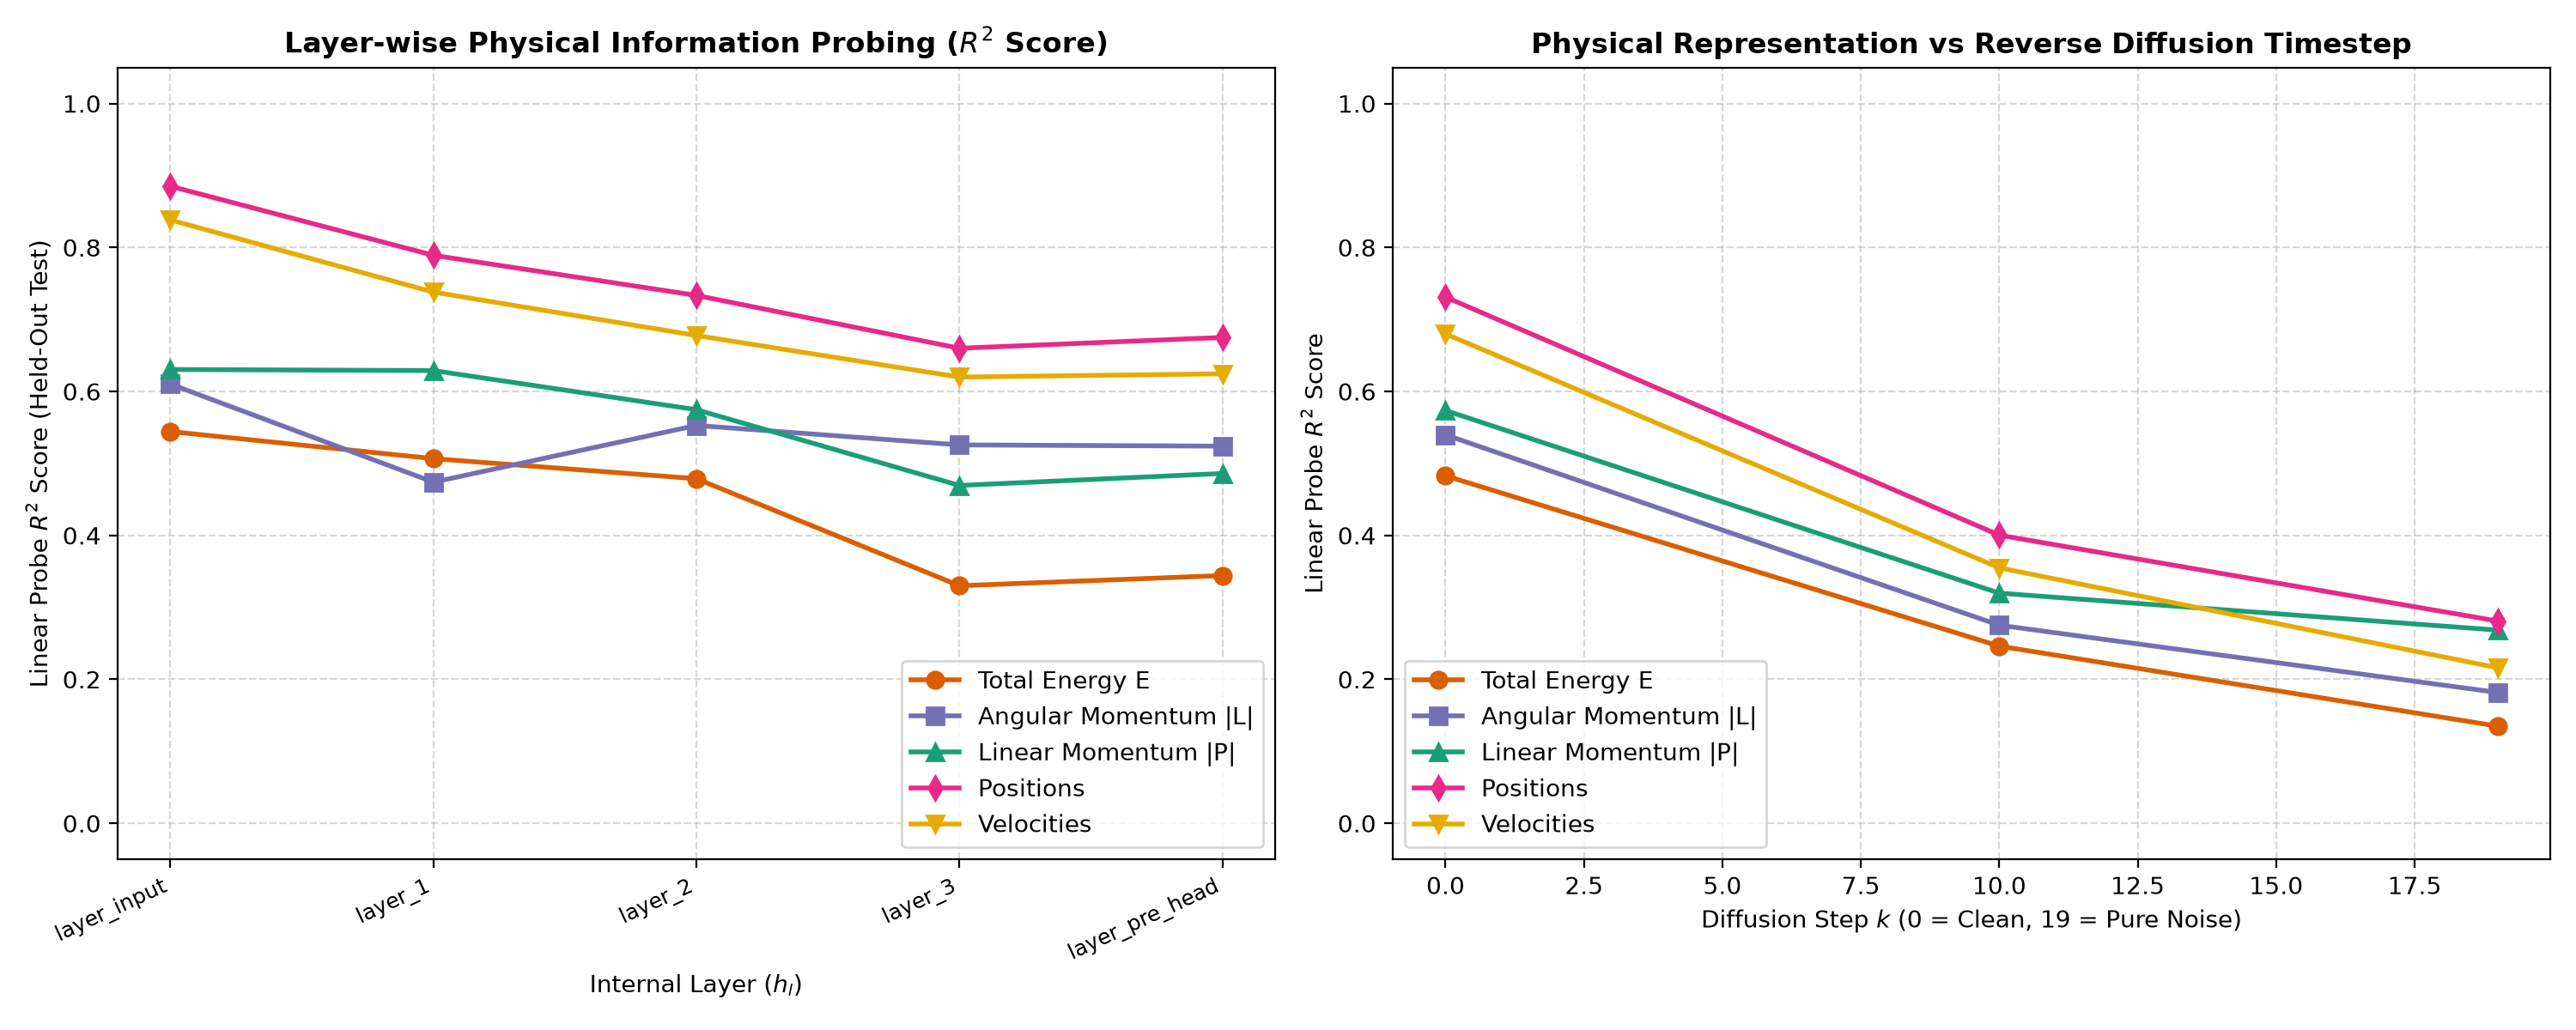
\includegraphics[width=\textwidth]{experiments_output/probing_results_layers.png}
        \caption{Layer-wise invariant probing and reverse diffusion crystallization.}
        \label{fig:probing_layers}
    \end{subfigure}
    \hfill
    \begin{subfigure}[b]{0.49\textwidth}
        \centering
        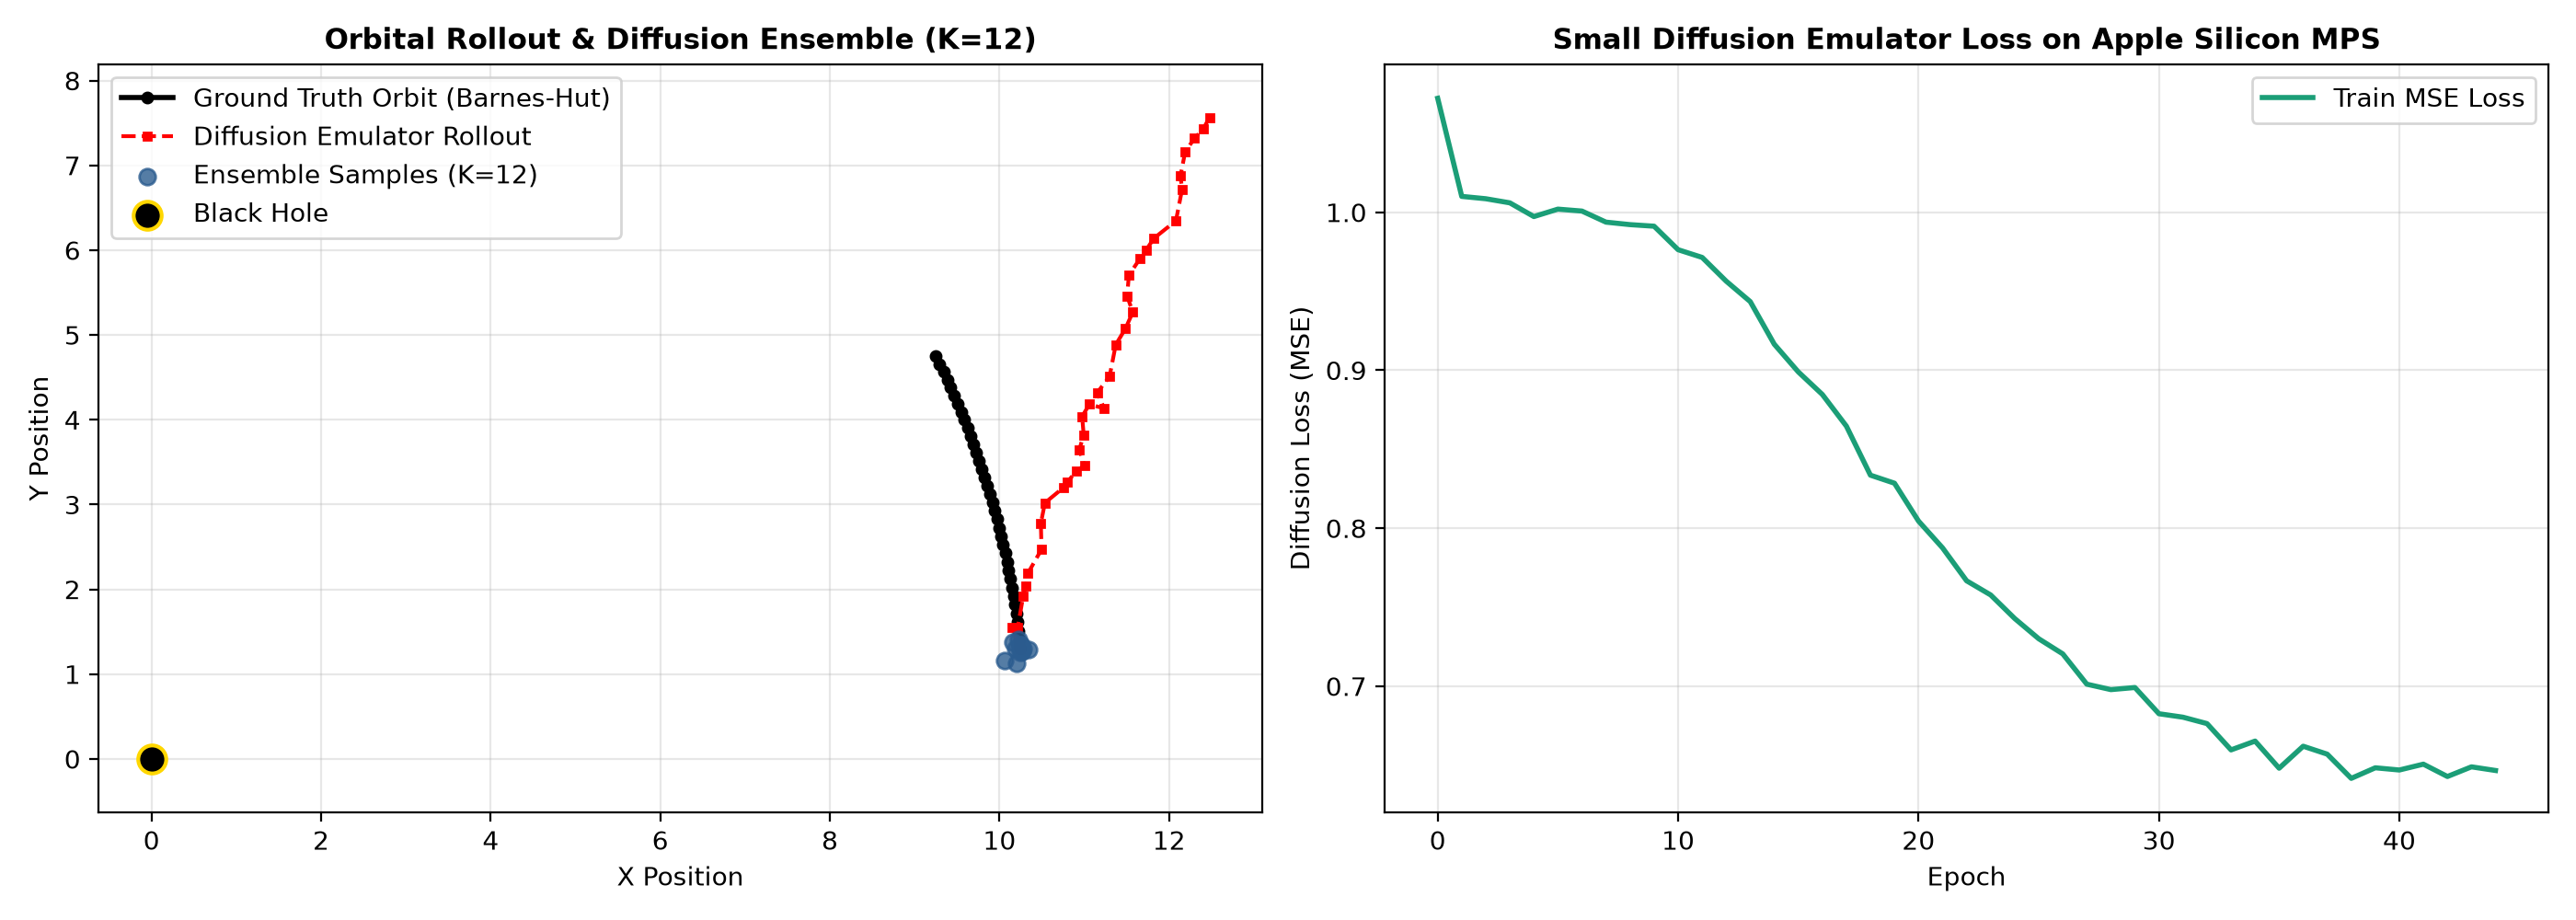
\includegraphics[width=\textwidth]{experiments_output/ensemble_rollout_comparison.png}
        \caption{Multi-step rollout and ensemble predictive spread.}
        \label{fig:ensemble_rollout}
    \end{subfigure}
    \caption{\textbf{Baseline Emulation \& Invariant Dynamics.} (a) Physical information accessibility across layers and reverse denoising steps $k = 19 \to 0$. (b) 2D orbit comparison against ground truth Barnes-Hut trajectory and training loss convergence.}
    \label{fig:baseline_panels}
\end{figure*}

\paragraph{Ensemble Predictive Spread.}
We sampled $S=8$ stochastic reverse diffusion trajectories per transition. As shown in Figure~\ref{fig:failure_probing} (bottom-right), ensemble predictive spread correlates only weakly with actual transition error ($r = 0.0402, \rho = 0.0317$), with a failure-to-success spread ratio of only $1.014\times$. While stochastic sampling reflects local diffusion variance, it does not reliably flag abrupt strong-field plunges near the ISCO, highlighting the complementary utility of internal representation probes.

\section{Discussion \& Conclusion}
In this work, we presented an empirical study of conditional diffusion models emulating pseudo-relativistic gravitational $N$-body systems. Our primary findings are:
\begin{enumerate}
    \item \textbf{Divergence of Representation Quality and Rollout Reliability:} Wider denoiser architectures systematically improve the linear accessibility of physical quantities ($R^2 > 0.93$ for angular momentum at $d=256$) and cut single-step training loss by $46.2\%$, but worsen 30-step autoregressive rollout RMSE from $6.966$ ($d=32$) to $18.465$ ($d=256$). This underscores that one-step objective optimization and long-horizon dynamical stability can diverge in unconstrained generative emulators.
    \item \textbf{Error Predictability from Internal Activations:} Hidden layer activations correlate with impending prediction error ($r = 0.6852$ at $h_{\mathrm{pre\_head}}$). While a substantial fraction of this correlation is explained by physical state difficulty (as confirmed by a physical baseline achieving $r = 0.7467$), probing residualized error shows that hidden features retain meaningful predictive capacity ($r = 0.4318$) beyond the input state.
    \item \textbf{Representation Breakdown During Failure:} Prediction failures are characterized by a $35.6\%$ reduction in coordinate decodability and an $11.9\%$ drop in angular momentum fidelity, associated with transitions entering strong-field regions near the ISCO.
\end{enumerate}

Importantly, our entire experimental workflow—from Barnes-Hut data generation to multi-model training and probing—executes in approximately 25 seconds on a base M1 MacBook Air, demonstrating that mechanistic interpretability for dynamical emulators can be conducted efficiently on local hardware. Future work will investigate incorporating symplectic Hamiltonian inductive biases directly into the diffusion score matching objective to mitigate autoregressive phase drift and improve long-horizon stability.

\bibliographystyle{plain}
\bibliography{references}

\end{document}
